\documentclass[11pt,a4paper]{article}
\usepackage[utf8]{inputenc}
\usepackage{amsmath}
\usepackage{amsfonts}
\usepackage{amssymb}

\title{The Gevo Times}


% Define geometry (without using the geometry package)
\setlength\topmargin{-48pt}
\setlength\headheight{0pt}
\setlength\headsep{0pt}
\setlength\marginparwidth{-20pt}
\setlength\textwidth{7.0in}
\setlength\textheight{9.5in}
\setlength\oddsidemargin{-30pt}
\setlength\evensidemargin{-30pt}

\setlength{\columnsep}{50pt}

\frenchspacing						% better looking spacing

% Call packages we'll need
\usepackage[english]{babel}			% english
\usepackage{graphicx}				% images
\usepackage{amssymb,amsmath}		% math
\usepackage{multicol}				% three-column layout
\usepackage{url}					% clickable links
\usepackage{marvosym}				% symbols
\usepackage{wrapfig}				% wrapping text around figures
\usepackage[T1]{fontenc}			% font encoding
\usepackage{charter} 				% Charter font for main content
\usepackage{blindtext}				% dummy text
\usepackage{datetime}				% custom date
	\newdateformat{mydate}{\THEMONTH. \THEYEAR}
\usepackage{librebaskerville}
\usepackage{helvet}

\usepackage[pdfpagemode=FullScreen, colorlinks=false]{hyperref}	% links and pdf behaviour
\usepackage[usenames,dvipsnames]{color} %using the color package, not xcolor



% Customize (header and) footer
\usepackage{fancyhdr}
\pagestyle{fancy}
\lfoot{	\footnotesize 
		The Gevo Times \\
		\Mundus\ \href{http://www.howtotex.com}{HowToTeX.com}	\quad
		\Telefon\ 555-5555											\quad
		\Letter\ \href{mailto:frits@howtotex.com}{frits@howtotex.com}
	  }
\cfoot{}
\rfoot{\footnotesize ~\\ Page \thepage}
\renewcommand{\headrulewidth}{0.0pt}	% no bar on top of page
\renewcommand{\footrulewidth}{0.4pt}	% bar on bottom of page

%%% ---------------
%%% DEFINITIONS
%%% ---------------

% Define separators
\newcommand{\HorRule}[1]{\noindent\rule{\linewidth}{#1}} % Creating a horizontal rule
\newcommand{\SepRule}{\noindent							 % Creating a separator
						\begin{center}
							\rule{250pt}{1pt}
						\end{center}
						}						

% Define Title en News input
% \renewcommand\familydefault{\sfdefault}  -helvetica default, ale není to hezké


\newcommand{\JournalName}[1]{%
		\begin{center}	
			\bfseries \Huge {The Gevo Times}
		\end{center}	
		\par \normalsize \normalfont}
		
\newcommand{\JournalIssue}[1]{%
		\hfill \textsc{\mydate \today, No #1} %vpravo nahoře
		\par \normalsize \normalfont}

\newcommand{\Nadpis}[1]{%
		\begin{center}
		{\bfseries	
		\Large #1 \vspace{4pt}
		\par \normalsize \normalfont}
		\end{center}}
		
\newcommand{\Podnadpis}[1]{
	%
	\begin{center}
	{
		\bfseries	
		\color{gray}
		\large #1 \vspace{2pt}
		%\par 
		\normalsize \normalfont
	}
	\end{center}
}
		
		
\newcommand{\NewsAuthor}[1]{
	%
	\bigbreak
	\hfill by \textsc{#1} \vspace{4pt}
	\par 
	\normalfont
}
			

			


%Defining colors
\definecolor{gray}{rgb}{0.4,0.4,0.4}
%%% ---------------
%%% BEGIN DOCUMENT
%%% ---------------
\begin{document}
% Title	
% -----
\JournalIssue{1}
\JournalName{The Gevo Times}
\noindent
{\color{gray} \rule{\linewidth}{1pt}} \\[-0.5\baselineskip]
%---------
\noindent\HorRule{3pt} \\[-0.63\baselineskip]
%-----
\noindent
{\color{gray} \rule{\linewidth}{1pt}} 
% -----
\begin{multicols}{2}
	\setlength{\columnseprule}{1pt}
	
%\nadpis 1
\Nadpis{Okénko třetích jazyků}

V tomto novém segmentu TGT se podíváme na
nedávnou akci ve světě třetích jazyků. (A ne
nejsou to výstupky) Jedná se o španělskou
olympiádu ve které jsme jako škola měli velmi
silné zastoupení. Standardně se pořádalo více
kol na jiných úrovních. My jsme dostali tu
možnost vyzpovídat výtěžku jednoho z nich a
také naší studentku Báru Bytnarovou.

\Podnadpis{Jak jsi se o této soutěži dozvěděla?}

Z ničeho nic za mnou přišla za mnou pani
profesorka Dimmerová a zeptala se mě jestli to
nechci zkusit. Tak jsem si řekla proč ne. Nic se
tím nezkazí a možná se i něco dozvím.

\Podnadpis{A dá se třeba říct, že ti to pomohlo do nadcházejících výstupek?}

Vzhledem k tomu, že to bylo velmi podobně
koncipováno tak se dá říct, že ano. Byla tam ta
poslouchací část, popis obrázku a gramatika.
Jediné co bylo nové byla reakce na nějakou
situaci. Obecně to bylo ovšem o hodně delší a
složitější.

\Podnadpis{Myslíš si, že bychom jen z hodin a malým samostudiem mohli dosáhnout na této olympiádě dobrých výsledků?}

Tak já osobně mám ve škole ještě hodiny navíc s
rodilým mluvčím kde se právě zaměřujeme na
mluvení. Ale nemyslím si, že s naší školní výukou
by studenti byli schopni uspět. Je to hlavně
dělané pro lidi které španělština baví takže dává
smysl, že to není pro každého.

\Podnadpis{Je někdo komu by jsi do příštích let doporučila účast na této olympiádě?}
Tak jestli Vám nedělali výstupky problém a cítíte se trochu jistí se svojí španělštinou tak to rozhodně má smysl. Jediné na co je třeba si dávat pozor tak v druhém kole se objevovaly i otázky zaměřené. Třeba na geografii jižní Ameriky.

\NewsAuthor{Jáchym Löwenhöffer}

\vspace{4ex}

%Nadpis 2
\Nadpis{ABC ěščřžýáíéúůĚŠČŘŽÝÁÍÉŮÚ eats frog}
\blindtext[1]
\Podnadpis{Fotka slona}
	\begin{center}
		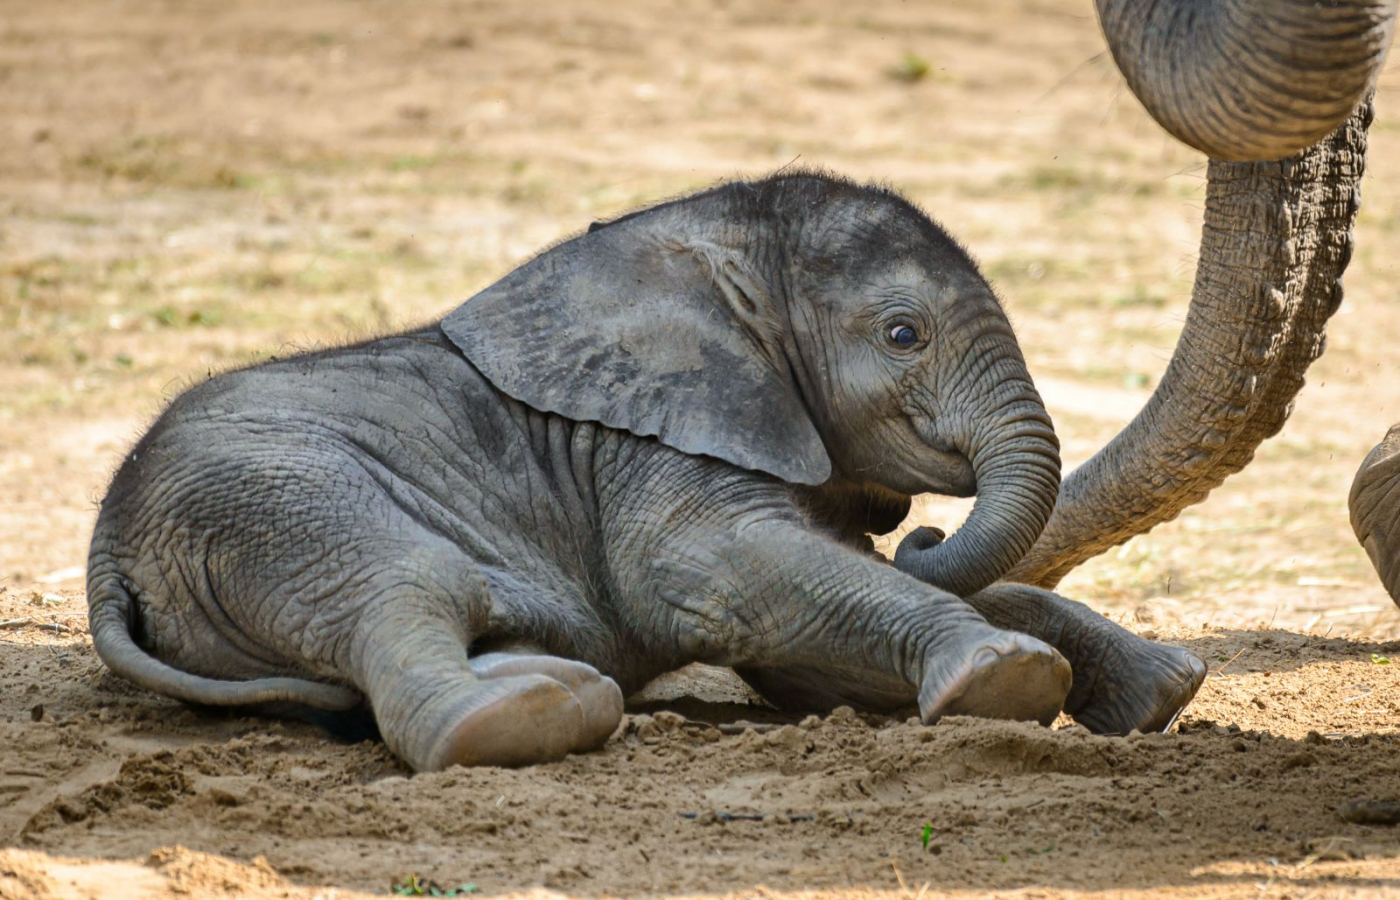
\includegraphics[width=0.8\linewidth]{elephant}
	\end{center}
\blindtext[1]
\NewsAuthor{J. Doe}
\end{multicols}
% -----
\end{document} 